\documentclass[sigconf]{acmart}

%%
%% \BibTeX command to typeset BibTeX logo in the docs
\AtBeginDocument{%
  \providecommand\BibTeX{{%
    \normalfont B\kern-0.5em{\scshape i\kern-0.25em b}\kern-0.8em\TeX}}}

%% Rights management information.
\setcopyright{rightsretained}
\copyrightyear{2026}
\acmYear{2026}
\acmDOI{XXXXXXX.XXXXXXX}

%% Conference information
\acmConference[L@S '26]{The 13th ACM Conference on Learning at Scale}{June 2026}{Location TBD}
\acmISBN{978-1-4503-XXXX-X/26/06}

\usepackage{array, tabularx}
\PassOptionsToPackage{hyphens}{url} % To allow URL breaking across lines

% Fix for arXiv missing acm-jdslogo and license icons
\makeatletter
\let\@notificationbox\relax
\let\ACM@cc@type\@empty
\makeatother

% If the error persists for acm-jdslogo, you can dummy it:
\newcommand{\acmJDSLogo}{}

\begin{document}

%%
%% Title
\title[Mitigating ``Epistemic Debt'' in GenAI-Scaffolded Novice Programming]{Mitigating ``Epistemic Debt'' in Generative AI-Scaffolded Novice Programming using Metacognitive Scripts}

%%
%% Authors (Anonymized for Double-Blind Review)
\author{Sreecharan Sankaranarayanan}
\affiliation{%
  \institution{Extuitive Inc. (Flagship Pioneering)}
  \city{Cambridge, Massachusetts}
  \country{United States of America}
}
\email{sreecharan.primary@gmail.com}

%%
%% Abstract (<350 Words)
\begin{abstract}
The democratization of Large Language Models (LLMs) has given rise to ``Vibe Coding'', a workflow where novice programmers prioritize semantic intent over syntactic implementation. While this lowers barriers to entry, we hypothesize that without pedagogical guardrails, it is fundamentally misaligned with cognitive skill acquisition. Drawing on Kirschner's (2026) distinction between \textit{Cognitive Offloading} and \textit{Cognitive Outsourcing}, we argue that unrestricted AI encourages novices to \textit{outsource} the Intrinsic Cognitive Load required for schema formation, rather than merely \textit{offloading} Extraneous Load. This accumulation of ``Epistemic Debt'' creates ``Fragile Experts'' — those whose high functional utility is masked by critically low corrective competence.

To quantify and mitigate this debt, we conducted a between-subjects experiment ($N=78$) using a custom Cursor IDE plugin backed by Claude 3.5 Sonnet. Participants were recruited via Prolific and UserInterviews.com to represent ``AI-Native'' learners. We compared three conditions: \textit{Manual} (Control), \textit{Unrestricted AI} (Outsourcing), and \textit{Scaffolded AI} (Offloading). The Scaffolded condition utilized a novel ``Explanation Gate,'' leveraging a real-time LLM-as-a-Judge framework to enforce a ``Teach-Back'' protocol before generated code could be integrated.

Results reveal a ``Collapse of Competence'': while Unrestricted AI users matched the productivity of the Scaffolded group ($p < .001$ vs. Manual), they suffered a 77\% failure rate in a subsequent AI-Blackout maintenance task, compared to only 39\% in the Scaffolded group. Qualitative analysis suggests that successful vibe coders naturally engage in self-scaffolding, treating the AI as a consultant rather than a contractor. We discuss the implications for the long-term maintainability of AI-generated software and propose that future learning systems must enforce \textit{Metacognitive Friction} to prevent the mass production of unmaintainable code. \footnote{Replication package (extension source, task suite, grading harness, and study protocol): \url{https://github.com/sreecharansankaranarayanan/vibecheck}}
\end{abstract}

%%
%% CSS Concepts
\begin{CCSXML}
<ccs2012>
    <concept>
        <concept_id>10003456.10003457.10003527</concept_id>
        <concept_desc>Social and professional topics~Computing education</concept_desc>
        <concept_significance>500</concept_significance>
    </concept>
    <concept>
        <concept_id>10010147.10010178</concept_id>
        <concept_desc>Computing methodologies~Artificial intelligence</concept_desc>
        <concept_significance>300</concept_significance>
    </concept>
    <concept>
        <concept_id>10003120.10003121</concept_id>
        <concept_desc>Human-centered computing~Human computer interaction (HCI)</concept_desc>
        <concept_significance>300</concept_significance>
    </concept>
</ccs2012>
\end{CCSXML}

\ccsdesc[500]{Social and professional topics~Computing education}
\ccsdesc[300]{Computing methodologies~Artificial intelligence}
\ccsdesc[300]{Human-centered computing~Human computer interaction (HCI)}

%%
%% Keywords
\keywords{Vibe Coding, Cognitive Outsourcing, Cognitive Offloading, Epistemic Debt, Script Theory of Guidance, Metacognitive Friction, Generative AI, Large Language Models, Computer Science Education, Software Engineering, Conversational Agents, Intelligent Tutoring Systems}

\maketitle

\section{Introduction}

A prevailing narrative in the technology sector suggests that software engineering as a discipline is nearing its end. Industry leaders and commentators have argued that with the advent of advanced Generative AI (GenAI), ``English is the new programming language'' \cite{world_governments_summit_2024_jensen_huang,karpathy2023english}, implying that the barrier to creating software has effectively dissolved. The assumption is that if AI can generate functional code from high-level natural language prompts—a practice colloquially known as \textbf{``Vibe Coding''} \cite{karpathy2024}—then the necessity for human expertise in syntax and logic is obsolete. Indeed, the long march of software engineering has moved toward abstracting away low-level details—from assembly programming to providing expressive power through language definitions closer to human natural language, such as Python. In that trajectory, treating human natural language as the next programming abstraction seems inevitable. However, from the standpoint of learning and the long-term maintainability of software, we posit a contrasting view.

While GenAI has undoubtedly democratized the creation of software, we hypothesize that unrestricted reliance on these tools, particularly in educational contexts, is engineering a latent crisis. If the next generation of developers learns to orchestrate ``vibes'' (intent) without understanding the underlying mechanics, we are not witnessing the democratization of engineering, but the accumulation of \textbf{Epistemic Debt}.

Epistemic Debt describes the accumulation of functional software artifacts that the user ``owns'' legally but does not ``own'' cognitively. Unlike technical debt, which resides in the codebase, epistemic debt resides in the \textit{mind} of the developer. When the inevitable abstraction leak occurs \cite{spolsky2002}—whether through API deprecation, hallucinated vulnerabilities, or scaling failures—the ``Vibe Coder'' lacks the mental model required to intervene. If this debt is not serviced during the learning process, the field faces a risk of a \textbf{``Collapse of Competence,''} where the workforce is replete with ``Fragile Experts'' who are skilled at adopting tools (high utility) but incapable of maintaining the systems they build (low comprehension).

Early hypotheses and evidence observing the over-reliance on GenAI in educational contexts have already started to question whether GenAI acts as a tool or is becoming a crutch \cite{balzan2026tools}. According to a CDT national poll, 70\% of teachers worry AI might weaken critical thinking and research skills, and more than half of students say they feel less connected to teachers when using AI tools \cite{laird2025hand}. Surveys regarding ChatGPT use just a year after its unveiling already raised fears that ``learners may rely too heavily on the model'' \cite{kasneci2023chatgpt}. Furthermore, ``diminished epistemic vigilance, superficial learning and emotional dependence on AI'' \cite{yan2025beyond}, as well as metacognitive laziness \cite{fan2025beware}, have been observed in specific studies. Indeed, students themselves report cognitive offloading and over-reliance on GenAI tools \cite{wei2025effects}. A useful metaphor to understand this phenomenon was posited by \citet{kirschner2026}: the distinction between cognitive offloading and cognitive outsourcing, founded in decades of cognitive and learning science research. On that basis, it is already possible to posit that our hypothesis, pointing to the accumulation of epistemic debt from the over-reliance on GenAI tools and the resulting competence collapse, will hold. Consequently, we must go a step further and ask whether this breakdown is inevitable.

The concern that technology-mediated shortcuts produce long-term skill atrophy is not novel to the GenAI era---it reflects a pattern that has surfaced repeatedly across prior generations of assistive technology. Bjork and Bjork's \textit{Desirable Difficulties} framework \cite{bjork2011desirable} and Ericsson et al.'s foundational work on deliberate practice \cite{ericsson1993} established that durable expertise is acquired through effortful, error-corrective struggle, not performance-optimized shortcuts. These dynamics were observed with pocket calculators, GPS navigators, and spell-checkers---tools that, deployed as substitutes for the underlying cognitive process rather than complements to it, were each found to correlate with atrophy in the very skills they were designed to assist \cite{kirschner2006minimal}. What distinguishes the present moment is both the breadth of GenAI's reach into cognitively demanding domains and the arrival of the first experimental confirmations of this pattern at scale. Bastani et al.~\cite{bastani2025} conducted a pre-registered randomized controlled trial with nearly 1,000 high school mathematics students and found that while unrestricted GPT-4 access improved practice performance by 48\%, it simultaneously reduced unassisted exam performance by 17\%---consistent with students substituting AI for the productive struggle that cements learning. In a parallel domain, Poulidis, Bastani, and Bastani~\cite{poulidis2025} ran a 12-week field experiment with over 200 chess club students, finding that self-regulated AI access---where students could request move hints on demand---produced less than half the skill gains of a system-regulated condition in which AI tips were algorithmically targeted to critical learning moments (30\% vs. 64\% improvement). Causal mediation analyses in that study confirmed that the performance gap was driven by the substitution of on-demand hints for productive struggle within each student's Zone of Proximal Development. Taken together, these findings across high school mathematics, chess training, and---as we demonstrate here---novice software engineering suggest that the deleterious effects of unscaffolded AI access may be a domain-general phenomenon rooted in the fundamental psychology of skill acquisition.

Can we design AI interactions and interventions that allow novices to leverage the speed and productivity benefits of GenAI tools without sacrificing the depth of their learning? In other words, can we arrive at a best-of-both-worlds scenario where high functional utility is achieved while learners retain enough expertise to produce comparable corrective competence?

To that end, we once again turn to learning science research, drawing inspiration from Teachable Agents \cite{biswas2005} to design an ``Explanation Gate'' intervention. This intervention requires novice learners, in a scaffolded setting, to teach-back what they have learned and understood to their AI chatbot before being allowed to use the generated code. We hypothesize that this introduction of ``Metacognitive Friction'' can restore learner comprehension without significantly degrading productivity. Our research questions are as follows:

Our research questions are as follows:

\begin{itemize}
    \item \textbf{RQ1 (Functional Utility \& Velocity):} To what extent does the introduction of automated metacognitive friction (the ``Explanation Gate'') impact the immediate functional utility and development velocity of novice programmers compared to unrestricted GenAI usage?
    \item \textbf{RQ2 (Corrective Competence \& Epistemic Debt):} Does unrestricted GenAI access lead to a collapse of competence in subsequent maintenance tasks, and can an explanation gate scaffold mitigate this accumulation of epistemic debt?
    \item \textbf{RQ3 (Interactional Stances):} What qualitative differences in human-AI interaction strategies (e.g., ``Consultant'' vs. ``Contractor'' stances) correlate with the retention of corrective competence in unrestricted GenAI environments?
\end{itemize}

Our contributions are as follows:
\begin{enumerate}
    \item \textbf{Theoretical Operationalization:} We define and operationalize the transition from Cognitive Offloading to Cognitive Outsourcing within the specific context of GenAI-assisted programming.
    \item \textbf{Empirical Quantification of Epistemic Debt:} We provide experimental evidence ($N=78$) demonstrating that while unrestricted AI preserves functional utility, it significantly degrades the corrective competence required for software maintenance.
    \item \textbf{Scalable Scaffolding Design:} We introduce and evaluate the \textit{VibeCheck} plugin, demonstrating that LLM-mediated metacognitive friction can restore human comprehension without significantly sacrificing AI-driven productivity gains.
    \item \textbf{Open Research Artifact:} We release the complete \textit{VibeCheck} extension, the Course Scheduler task suite (starter scaffold, reference implementation, and logic bomb version), the 12-assertion grading harness, and the full three-condition study replication protocol as an open artifact.\footnote{\url{https://github.com/sreecharansankaranarayanan/vibecheck}}
\end{enumerate}

\section{Theoretical Framework}

Our investigation is grounded in a synthesis of three complementary theories of learning: Cognitive Load Theory (specifically the distinction between Offloading and Outsourcing) \cite{sweller1988}, the Script Theory of Guidance (SToG) \cite{fischer2013}, and the ``Desirable Difficulties" framework \cite{bjork1994}. We argue that the interaction between novice programmers and Large Language Models (LLMs) represents a novel pedagogical context where traditional scaffolding metaphors break down, requiring a re-evaluation of how automated assistance supports, or subverts, schema acquisition.

\subsection{Cognitive Load: Offloading vs. Outsourcing}
A critical error in current EdTech discourse is the conflation of efficiency (productivity) with learning (schema construction). To dismantle this, we rely on Sweller's Cognitive Load Theory \cite{sweller1988}, specifically the interplay between three types of load:
\begin{enumerate}
    \item \textbf{Intrinsic Load:} The inherent complexity of the material (e.g., control flow logic, variable state).
    \item \textbf{Extraneous Load:} The mental effort imposed by the instructional format (e.g., confusing syntax, IDE configuration).
    \item \textbf{Germane Load:} The mental effort dedicated to processing information into Long-Term Memory (LTM) schemas.
\end{enumerate}

Expert developers use tools to minimize Extraneous Load, freeing up working memory for high-level problem solving (Germane Load). Kirschner \cite{kirschner2026} defines this as \textbf{Cognitive Offloading}. However, novices lack the schemas to distinguish between syntax (extraneous) and logic (intrinsic). When a novice uses GenAI to Vibe Code, the tool handles both the syntax and the underlying logic. This transition from \textit{Offloading} to \textbf{Cognitive Outsourcing} allows the learner to bypass the Intrinsic Load entirely \cite{kirschner2026}. Without engaging with Intrinsic Load, Germane processing cannot occur, and the learner accumulates epistemic debt, a state where functional output exists without the corresponding mental models to maintain it.

\subsection{Overscripting}
Fischer's Script Theory of Guidance (SToG) posits that external scripts (prompts, roles, instructions) are necessary to help learners coordinate complex tasks \cite{fischer2013}. Ideally, these scripts provide a temporary structure that is gradually ``faded" as the learner's internal scripts (schemas) mature \cite{wecker2010fading}.

We argue that the ``Copy-Paste" AI workflow represents a pathological case of \textbf{Overscripting} \cite{dillenbourg2002over}. Because standard LLMs provide complete, high-fidelity solutions instantly, they act as a rigid script that replaces, rather than regulates, the learner's cognitive activity. Unlike human tutors who withhold answers to prompt reflection, an unrestricted LLM resolves the problem space immediately, denying the learner the ``productive failure" necessary for transfer \cite{kapur2008productive}.

To counteract this, we introduce the concept of \textbf{Metacognitive Friction}. This design paradigm deliberately slows down the interaction loop, forcing the learner to engage in generative processing. This aligns with Bjork's concept of \textit{Desirable Difficulties} \cite{bjork1994}, specifically the ``Generation Effect," which posits that long-term retention is improved when learners must actively retrieve and reformulate knowledge rather than passively consuming it.

\subsection{Scalable Assessment as the Gatekeeper}
Historically, the Teachable Agent paradigm, where students learn by teaching a computer agent, has been shown to be highly effective for deep learning \cite{biswas2005}. However, verifying that a student has truly ``taught" the agent (rather than gaming the system \cite{baker2005designing}) traditionally required human Teaching Assistants (TAs), limiting the scalability of such interventions.

Recent advancements in LLM-Based Assessment allow us to automate this verification at scale. By leveraging an ``LLM-as-a-Judge'' framework \cite{choma2025}, we can convert the Teachable Agent model into a real-time ``Explanation Gate.'' This system acts as a semantic validity check, ensuring that the learner's vibe (intent) is backed by sufficient syntactic understanding before code integration is permitted. This effectively closes the loop on Outsourcing, forcing the learner to convert the AI's output back into their own internal representation before moving forward.

\section{Methodology}

\subsection{Participants \& Recruitment}
We recruited $N=78$ participants located in the United States for a 2-hour synchronous remote session. To ensure a representative sample of AI-Native learners, we utilized a dual-channel sourcing strategy to capture both traditional students and vocational learners:

\begin{enumerate}
    \item Prolific ($n=53$): Targeting current undergraduate students majoring in Computer Science or related STEM fields.
    \item UserInterviews.com ($n=25$): Targeting recent graduates ($<12$ months) of intensive coding bootcamps to capture the vocational segment.
\end{enumerate}

\textbf{Screening Criteria:} Participants were screened for basic familiarity with JavaScript (i.e., they could write a loop and define a function) but no professional experience with React.js (the target framework).

\textbf{Demographics:} The sample was 34\% female, 64\% male, and 2\% non-binary. While we attempted to stratify for gender balance, the pool reflected the broader demographics of the sourcing platforms and the domain. The mean age was 22.1 years ($SD=1.8$, Range=19--29). All participants were compensated at a rate of \$15 USD/hour.

\subsection{The Coding Environment}
We developed a custom experimental environment to mimic a real-world Vibe Coding setup while maintaining experimental control.

\begin{itemize}
    \item \textbf{IDE:} All participants used Cursor IDE, a fork of VS Code that integrates LLM features natively.
    \item \textbf{Generator Model:} We utilized Claude 3.5 Sonnet (via API) for all code generation, chosen for its dominance in coding benchmarks as of the time this study was conducted in Fall 2025 \cite{anthropic2024claude35sonnet}.
    \item \textbf{Plugin Architecture:} We developed a custom VS Code extension, \textit{VibeCheck} \footnote{\url{https://github.com/sreecharansankaranarayanan/vibecheck}}, which acted as a middleman between Cursor's AI agent and the file system. As illustrated in Figure \ref{fig:arch}, the extension implemented three core logic layers:
    \begin{enumerate}
        \item \textbf{Rule Enforcement Engine:} A document-change listener (\texttt{onDidChangeTextDocument}) that detected large AI-generated writes (threshold: $\geq$2 lines or $\geq$50 characters) using a per-document snapshot of the last human-authored state. Rather than fighting Cursor's agent in-memory—where the AI actively re-applies undone changes—the engine used VS Code's \texttt{onWillSaveTextDocument} hook to intercept file persistence (see Figure~\ref{fig:notifications}, left). By injecting TextEdit operations that restored the pre-AI snapshot before each disk write, the engine ensured that no AI-generated code persisted until the gate was satisfied. A secondary \texttt{onDidSaveTextDocument} fallback handled cases where Cursor's native ``Keep Changes'' diff UI wrote files outside VS Code's standard save pipeline, immediately overwriting any unauthorized disk write with the checkpoint content. For Group A (Manual), clipboard paste events exceeding 20 characters from external sources triggered a warning flag.
        \item \textbf{Explanation Gate Manager (The Friction Loop):} A per-document state machine (\texttt{idle} $\to$ \texttt{gating} $\to$ \texttt{blocked/approved}) responsible for the intervention. Upon detecting a halted write, this manager rendered a blocking WebView panel (Figure \ref{fig:gate_ui}) displaying the intercepted code snippet. It orchestrated an asynchronous loop with the \textbf{Judge API}, preventing file persistence until the Judge returned a ``Pass'' evaluation. If the gate was cancelled, a ``Try Again'' notification restored the gating state with the original snippet, re-opening the panel without requiring the student to re-trigger a Cursor AI action.
        \item \textbf{Telemetry Logger:} Recorded every gate encounter, explanation attempt, Judge score, and state transition with millisecond-precision timestamps for post-hoc analysis.
    \end{enumerate}
\end{itemize}

\begin{figure}[ht]
  \centering
  \Description{System architecture flowchart showing input from Sidebar and Keystrokes being processed by Rule Enforcement Engine and potentially gated by the Explanation Gate Manager.}
  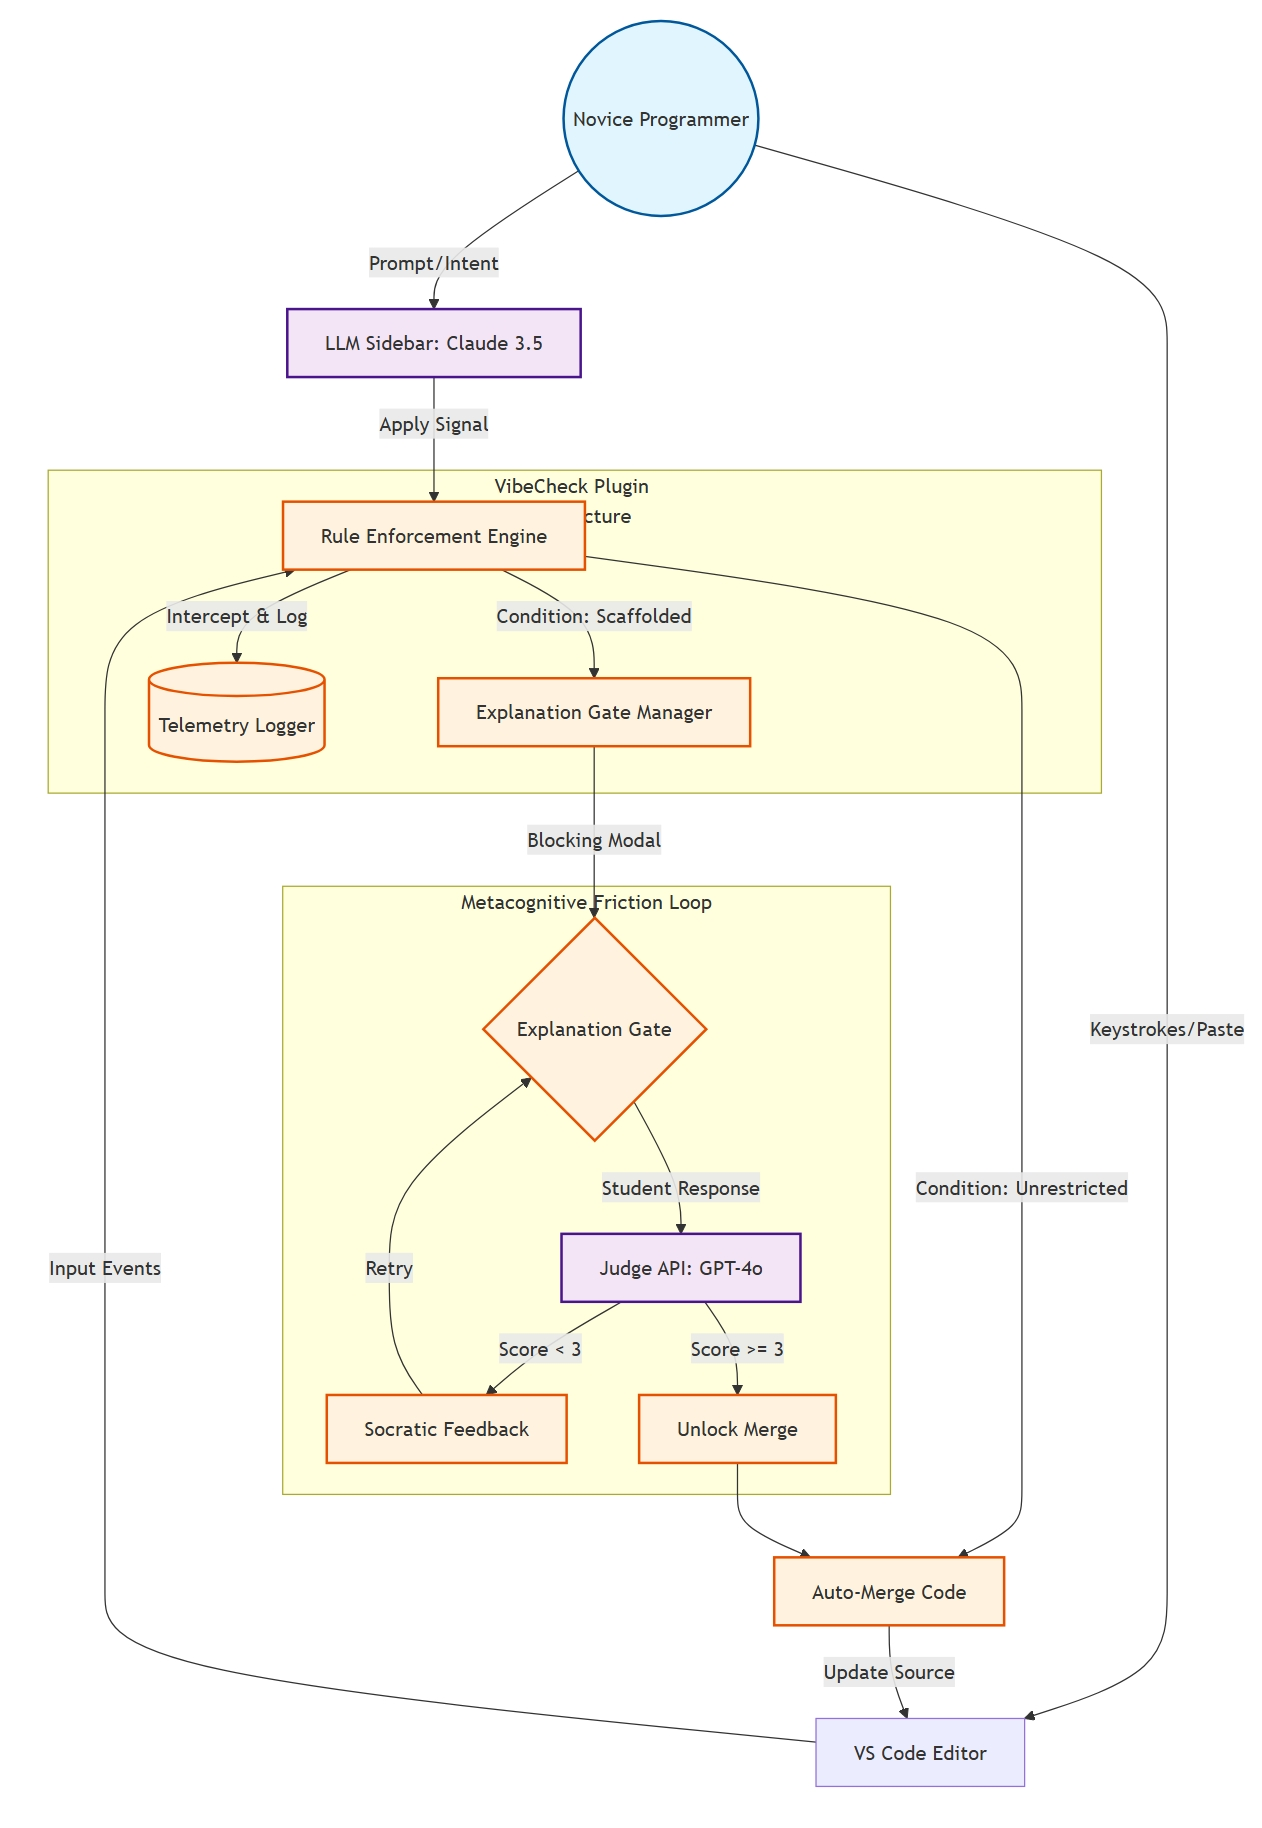
\includegraphics[width=\linewidth]{vibecheck_mermaid_live.jpeg}
  \caption{System Architecture of the \textit{VibeCheck} Plugin. The diagram illustrates how the Rule Enforcement Engine intercepts the ``Apply'' signal from the LLM Sidebar and conditionally routes it through the Explanation Gate Manager, enforcing a Metacognitive Friction loop via the external Judge API.}
  \label{fig:arch}
\end{figure}

\subsubsection{The ``Judge'' Agent}
To enable scalable assessment, the Explanation Gate utilized a secondary LLM agent to evaluate student explanations in real-time. We selected GPT-4o (OpenAI) as the judge to minimize self-preference bias (where a model prefers its own output style) \cite{wataoka2024self,chen2025beyond}. The judge was configured with a temperature of \textnormal{\texttt{0.1}} to ensure deterministic grading.

\textbf{System Prompt:} The judge was initialized with the following rubric based on the SOLO Taxonomy \cite{biggs1989towards}:

\begin{quote}
{\itshape You are a Teaching Assistant for a React course. Your goal is to evaluate if the student truly understands the code they are trying to merge. 
\newline
\textbf{Context:} The student has generated code using AI and must explain it to you.
\newline
\textbf{Rubric:} Grade their explanation on a scale of 1-5:
\begin{itemize}
    \item 1 (Pre-structural): Tautological (e.g., \textnormal{\texttt{It adds the button}}).
    \item 3 (Relational): Explains how components interact (e.g., \textnormal{\texttt{It uses the state hook to update the list}}).
    \item 5 (Extended Abstract): Explains edge cases or architectural impact.
\end{itemize}
\textbf{Output:} JSON format \textnormal{\texttt{\{ "score": number, "feedback": string \}}}. If score < 3, provide specific, Socratic feedback to guide them (e.g., \textnormal{\texttt{You mentioned state, but how does the useEffect dependency array affect the update loop?}}). Do not reveal the answer.}
\end{quote}

The student saw the modal prompt: \textit{``Wait! Before applying this code, explain its causal logic. How does it handle state updates?''} If the Judge returned a score below 3, the modal remained locked, displaying the Judge's Socratic feedback. This cycle repeated until a passing score was achieved. Figure \ref{fig:gate_ui} shows the gate panel as presented to participants.

\begin{figure}[ht]
  \centering
  \Description{Screenshot of the VibeCheck Explanation Gate panel showing a code snippet in a read-only preview area and a textarea prompting the student to explain the causal logic before the code is applied.}
  
\includegraphics[width=0.92\linewidth]{vibecheck_gate_ui.png}
  \caption{The VibeCheck Explanation Gate panel. The intercepted code snippet is shown in a read-only preview; the student must submit a SOLO Level 3+ explanation before the code is saved to disk. Attempt number, real-time Judge feedback, and score are displayed inline.}
  \label{fig:gate_ui}
\end{figure}

\begin{figure}[ht]
  \centering
  \Description{Two VS Code notification toasts produced by VibeCheck. Left: an amber warning reading ``VibeCheck: Edit reverted — explain code to apply'' shown whenever a Cmd+S or auto-save is attempted while the gate is unresolved. Right: a blocking amber warning reading ``VibeCheck: Changes blocked — explain the code to apply it'' with a ``Try Again'' action button, shown when the student dismisses the Explanation Gate without passing.}
  \begin{minipage}{0.48\linewidth}
    
\includegraphics[width=\linewidth]{edit_reverted.png}
  \end{minipage}\hfill
  \begin{minipage}{0.48\linewidth}
    
\includegraphics[width=\linewidth]{dismiss_gate.png}
  \end{minipage}
  \caption{VS Code notification feedback loop. \textbf{Left}: an ``Edit reverted'' toast appears on every blocked save attempt, reminding the student that the gate is pending. \textbf{Right}: a ``Changes blocked'' toast with a ``Try Again'' action is shown when the gate is dismissed, allowing the student to re-open the panel with the same code snippet without re-triggering Cursor's AI.}
  \label{fig:notifications}
\end{figure}

The use of the SOLO taxonomy for evaluating student explanations was derived with the help of an expert learning designer as the human-in-the-loop using the process described in \citet{choma2025}.

\begin{table}[ht]
  \caption{SOLO Taxonomy Calibration for Automated Judge Evaluation}
  \label{tab:solo_calibration}
  \small
  \begin{tabularx}{\columnwidth}{c|c|X}
    \toprule
    \textbf{Score} & \textbf{SOLO Level} & \textbf{Student Explanation Example} \\
    \midrule
    1 & Pre-structural & ``I added a button so that when you click it the course is added to the list and it updates.'' \\
    \hline
    2 & Unistructural & ``It uses the \texttt{enrollCourse} function to send the ID to the database and then changes the UI.'' \\
    \hline
    3 & \textbf{Relational} & ``The \texttt{await} keyword ensures the app waits for the DB confirmation before updating the local \texttt{courses} state, preventing UI desync.'' \\
    \hline
    5 & Ext. Abstract & ``It implements optimistic updates by updating the state first but uses a \texttt{try/catch} to rollback the UI if the fetch request fails, ensuring eventual consistency.'' \\
    \bottomrule
  \end{tabularx}
\end{table}

Figure \ref{fig:score_examples} illustrates representative gate interactions at SOLO Levels 1 and 2, showing the Socratic feedback the Judge returned in each case. The most common failure mode (Pre-structural, score 1) was a tautological restatement of the task description with no causal content; the second most common (Unistructural, score 2) identified a single relevant element (e.g., a component or function name) without explaining the interaction between components.

\begin{figure}[ht]
  \centering
  \Description{Two side-by-side screenshots of the VibeCheck gate showing Score 1/5 and Score 2/5 feedback from the Judge API, illustrating the two most common failure modes.}
  \begin{minipage}{0.48\linewidth}
    
\includegraphics[width=\linewidth]{score_1_5.png}
  \end{minipage}\hfill
  \begin{minipage}{0.48\linewidth}
    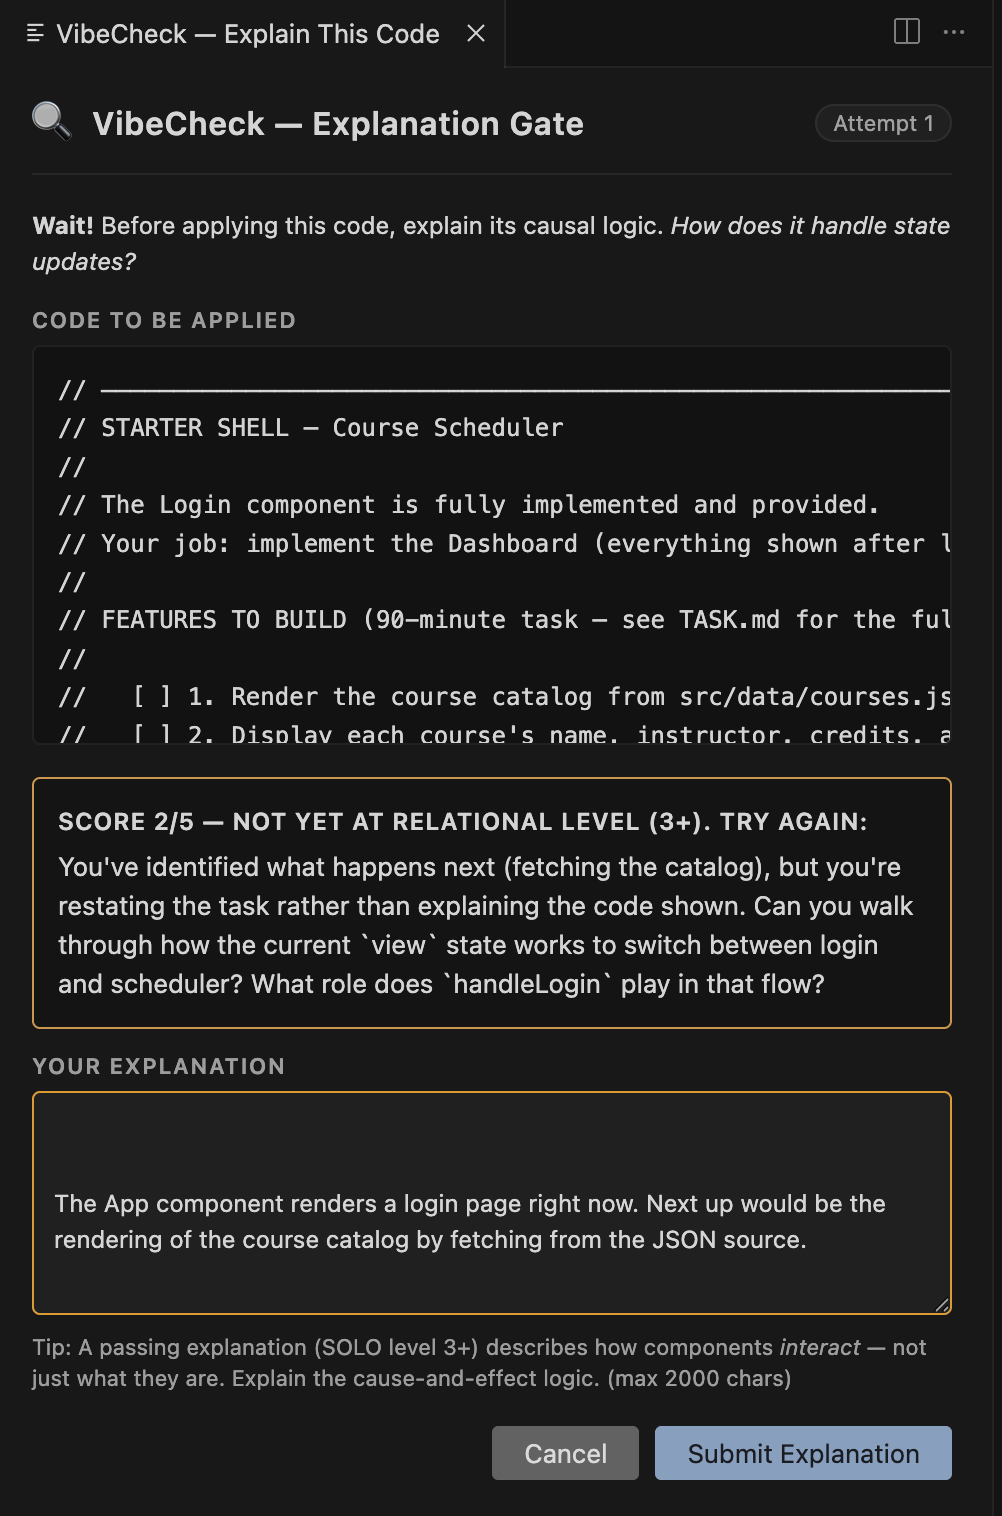
\includegraphics[width=\linewidth]{score_2_5.png}
  \end{minipage}
  \caption{Representative gate interactions at SOLO Levels 1 (left) and 2 (right). Score 1 responses restate the task prompt without causal content; Score 2 responses identify a single element but omit component interaction. In both cases the Judge returns targeted Socratic questions rather than revealing the answer, guiding the student toward a Relational (Level 3) explanation.}
  \label{fig:score_examples}
\end{figure}

\subsection{Experimental Conditions}
Participants were assigned via a Stratified Randomization protocol. Within each recruitment channel, participants were randomly assigned to one of three conditions to ensure equal distribution ($n=26$ per group).

\subsubsection{Group A: Manual (Control)}
Participants used the standard VS Code environment. They had access to official React documentation but were strictly forbidden from using Generative AI tools.

\textbf{Enforcement:} The \texttt{VibeCheck} Rule Enforcement Engine monitored clipboard events; paste events exceeding 20 characters from external sources triggered a warning flag. Additionally, screen recordings of a random 10\% sample were manually reviewed for compliance.

\subsubsection{Group B: Unrestricted AI (Outsourcing)}
Participants used Cursor IDE with free access to Claude 3.5 Sonnet in the sidebar. The Apply button was enabled instantly. This feature automatically diffs and merges generated code into the active file, mimicking the default Vibe Coding experience.

\subsubsection{Group C: Scaffolded AI (Offloading)}
Participants used Cursor IDE with the extension active. The Apply button was disabled by default. To unlock it, the Explanation Gate Manager triggered a modal asking: \textit{``Explain the causal logic of this block. How does it handle state updates?''}

\textbf{The Judge:} The student's response was sent to a background GPT-4o agent. We purposefully selected a model family different from the generator (Claude) to minimize self-preference bias in evaluation, as explained in the previous section.

\textbf{Feedback Loop:} If rejected, the student received the feedback (e.g., ``You identified \textit{what} variables are used, but not \textit{why} the effect hook is needed here'') and had to retry.

\subsection{Task Protocol}
The experiment consisted of two distinct phases designed to evaluate the trade-off between the immediate production of software and the long-term acquisition of learner competence.

\subsubsection{Phase 1: Functional Utility}
Over a 90-minute period, participants were tasked with building a ``Student Course Scheduler'' React application. This phase was designed to measure \textbf{Functional Utility}. The application requirements included:
\begin{enumerate}
    \item \textbf{Authentication:} A functional mock login interface.
    \item \textbf{Data Rendering:} Displaying course metadata from a provided JSON source.
    \item \textbf{Stateful Enrollment:} Implementing a selection system to add courses.
    \item \textbf{Conflict Logic:} Algorithmic detection to prevent overlapping schedules.
\end{enumerate}

During this phase, the \textbf{Rule Enforcement Engine} and \textbf{Explanation Gate Manager} were active. For Group C, every attempt to integrate logic triggered the Metacognitive Friction loop, requiring a passing explanation before code could be merged. 

\textbf{Primary Metric:} The \textit{Functional Utility Score} (0–100), calculated via a headless Puppeteer/Jest test harness that executed 12 end-to-end assertions. Each assertion was weighted equally (8.33 points).

\begin{table}[ht]
    \small
    \caption{12 Component Assertions of the Functional Utility Score for a Total of 100 Points}
    \label{tab:func_util}
    \begin{tabularx}{\columnwidth}{l|X}
        \toprule
        \textbf{ID} & \textbf{Assertion Description} \\
        \midrule
        A-01 & User can log in using mock credentials and reach the dashboard. \\
        A-02 & Course catalog successfully fetches and renders 20+ items from JSON. \\
        A-03 & Course list displays correct metadata (Instructor, Credits, Time). \\
        A-04 & Clicking ``Enroll'' adds a course to the user's sidebar state. \\
        A-05 & Duplicate enrollment in the same course is blocked by state logic. \\
        A-06 & The system identifies time-overlaps between two distinct courses. \\
        A-07 & A warning modal appears when a conflict is detected. \\
        A-08 & Total credit count updates dynamically as courses are added/removed. \\
        A-09 & Enrollment persistence: data remains after simulated page refresh. \\
        A-10 & Search functionality filters the course catalog by name/instructor. \\
        A-11 & Conflict detection logic correctly handles back-to-back classes. \\
        A-12 & Final schedule export generates a valid summary string. \\
        \bottomrule
    \end{tabularx}
\end{table}

\subsubsection{Phase 2: Corrective Competence}
Immediately following Phase 1, we simulated an ``abstraction leak'' to measure the participants' \textbf{Corrective Competence}. AI access was revoked for all groups, and we used a git patch to inject a \textbf{Logic Bomb} into their functioning codebase.

We introduced a race condition in the \texttt{enrollCourse} function by stripping the \texttt{await} keywords from asynchronous database calls and deleting the optimistic UI rollback logic. Under simulated network latency, the UI would optimistically show a course as added, but the underlying state would fail to sync, causing the course to vanish upon browser refresh (a ``ghost course''). Participants were given the final 30 minutes to identify the cause of the ghost courses and manually implement a fix without AI assistance.

It is important to distinguish between general debugging and the measurement of \textit{Corrective Competence}. To ensure we were measuring the latter, the Logic Bomb was not a novel bug, but a structural regression of the participant's \textit{own existing code}. Because all participants in Groups B and C had successfully implemented a functional enrollment system in Phase 1 (verified by the test harness), they had all previously ``owned'' a version of the code where the asynchronous \texttt{await} and rollback logic were present. Thus, the Phase 2 task did not require the discovery of a new architectural pattern, but rather the recognition and restoration of a logic flow they had ostensibly integrated already prior. Failure to resolve this regression served as a direct proxy for the Epistemic Debt accumulated during the initial construction.

\textbf{Primary Metric:} \textit{Corrective Competence}, measured as a binary Repair Success (resolved vs. unresolved) and Time-to-Fix.

\begin{table}[ht]
  \caption{The Phase 2 ``Logic Bomb'' Regression}
  \label{tab:logic_bomb}
  \small
  \begin{tabularx}{\columnwidth}{X|X}
    \toprule
    \textbf{Original (Functional)} & \textbf{Injected Regression (Bug)} \\
    \midrule
    \texttt{const res = await fetch('/enroll');} & \texttt{const res = fetch('/enroll');} \\
    \texttt{if (res.ok) \{ updateUI(); \}} & \texttt{updateUI(); // Optimistic} \\
    \texttt{else \{ rollback(); \}} & \texttt{// No rollback logic} \\
    \bottomrule
  \end{tabularx}
\end{table}

\section{Results}

Our analysis evaluates the experimental data through the lens of the trade-off between immediate software production (Utility) and the acquisition of long-term learner competence. 

\subsection{RQ1: Functional Utility and Velocity}
To evaluate whether the Metacognitive Friction of the Explanation Gate significantly impeded immediate software production, we analyzed both the Phase 1 Functional Utility Scores and the total time spent on the construction task.

\subsubsection{Functional Utility}
We verified the assumptions for parametric testing; normality was confirmed using a Shapiro-Wilk test ($W = 0.98, p = .42$), and homogeneity of variance via Levene's test ($F(2, 75) = 1.12, p = .33$). A one-way ANOVA revealed a highly significant effect of condition on utility ($F(2, 75) = 48.2, p < .001, \eta^2 = 0.56$).

As detailed in Table \ref{tab:phase1}, both AI-assisted groups achieved significantly higher utility than the manual control. Post-hoc Tukey HSD tests revealed no significant difference in functional utility between the Unrestricted and Scaffolded groups ($p = .64$).

\begin{table}[ht]
  \caption{Phase 1: Functional Utility Scores}
  \label{tab:phase1}
  \begin{tabular}{ccl}
    \toprule
    Condition & Mean Utility Score & SD\\
    \midrule
    Manual (Group A) & 65.2\% & 14.3\\
    Unrestricted AI (Group B) & 92.4\% & 8.1\\
    Scaffolded AI (Group C) & 89.1\% & 9.5\\
    \bottomrule
  \end{tabular}
\end{table}

\subsubsection{Development Velocity and Cognitive Allocation}
To evaluate the ``velocity cost'' of metacognitive friction, we compared total time-on-task and the allocation of \textit{Active Thinking} time. We define Active Thinking as the duration spent in manual construction, code comprehension, and, for Group C, the duration of Explanation Gate interventions. 

As shown in Table \ref{tab:time_results}, the progress metric reveals that the Manual group exhausted the 90-minute limit having only satisfied 42\% of the requirements. In contrast, both AI-enabled groups achieved 100\% completion. 

While the Scaffolded group encountered a significant velocity penalty compared to the Unrestricted group ($p < .001$), their ``Net Velocity'' remained superior to the Manual control. The friction introduced by the Explanation Gate (Median = 14.2 minutes) was effectively subsidized by the generational speed of the LLM. 

\newcolumntype{C}{>{\centering\arraybackslash}X}

\begin{table}[ht]
  \caption{Phase 1: Time on Task and Cognitive Allocation}
  \label{tab:time_results}
  \small
  \begin{tabularx}{\columnwidth}{lCCC}
    \toprule
    Condition & Total Time Mean ($SD$) & Active Thinking Mean ($SD$) & Progress (\%)\\
    \midrule
    Manual (A) & 88.4 (2.1) & 88.4 (2.1) & 42\%\\
    Unrestricted (B) & 48.2 (10.4) & 18.5 (4.2) & 100\%\\
    Scaffolded (C) & 64.6 (11.2) & 36.3 (5.8) & 100\%\\
    \bottomrule
  \end{tabularx}
\end{table}

\subsection{RQ2: Corrective Competence and Epistemic Debt}
In Phase 2, we measured the \textit{Corrective Competence} of participants after AI access was revoked. Repair Success rates for the race-condition logic bomb were analyzed using a Chi-square test of independence, yielding significant results ($\chi^2(2) = 13.8, p = .001, V = 0.42$).

\begin{itemize}
    \item \textbf{Manual (Group A):} 18/26 succeeded (\textbf{69.2\%}). Despite lower initial utility, these participants possessed high cognitive ownership.
    \item \textbf{Unrestricted AI (Group B):} 6/26 succeeded (\textbf{23.1\%}). This group exhibited a clear Collapse of Competence. 
    \item \textbf{Scaffolded AI (Group C):} 16/26 succeeded (\textbf{61.5\%}). The ``Explanation-Gate'' successfully mitigated the accumulation of epistemic debt.
\end{itemize}

\subsection{RQ3: Interactional Stances}
We investigated the \textbf{6 participants} in Group B who successfully fixed the bug. We identified two distinct behaviors:
\begin{enumerate}
    \item \textbf{The Contractor Stance:} Prompts focused on functional output.
    \item \textbf{The Consultant Stance:} Successful outliers consistently prompted for clarification.
\end{enumerate}

Successful participants utilized a mean of 4.2 explanatory prompts per session, compared to 0.4 for those who failed ($t(24) = 5.1, p < .001$). 

\begin{table*}[ht]
  \caption{Representative Individual Results showing the divergence in Phase 2.}
  \Description{Table showing Phase 1 utility scores against Phase 2 repair results and time to fix across different conditions and participant IDs.}
  \label{tab:individual}
  \begin{tabular}{llcllc}
    \toprule
    ID & Condition & Utility (Ph 1) & Repair Result (Ph 2) & Fix Time & Dominant Stance (Ph 1)\\
    \midrule
    P-12 & Manual & 72\% & Success & 11m 45s & Manual Reasoning\\
    P-23 & Unrestricted & 95\% & Fail & Timeout & Contractor (Directive)\\
    P-35 & Unrestricted & 98\% & Success & 21m 10s & Consultant (Explanatory)\\
    P-48 & Scaffolded & 90\% & Success & 13m 30s & Enforced Consultant\\
    P-55 & Scaffolded & 82\% & Fail & Timeout & Tautological (Low SOLO)\\
    \bottomrule
  \end{tabular}
\end{table*}

\subsection{The Consultant vs. The Contractor}
Our analysis of the interaction logs in Group B (Unrestricted) reveals a critical behavioral predictor of corrective competence. We identified two dominant interactional stances:

\begin{description}
    \item[\textbf{The Contractor Stance:}] These participants treated the LLM as a low-level worker. Prompts were purely imperative (e.g., ``Make the button blue,'' ``Add the filter''). Telemetry shows these users rarely scrolled through the generated code before clicking ``Apply.'' This stance maximize immediate velocity but results in 100\% Cognitive Outsourcing.
    \item[\textbf{The Consultant Stance:}] Outliers who succeeded in Phase 2 treated the LLM as a senior partner. Their prompts were interrogative (e.g., ``Why did you use a useEffect here?'' or ``Can you explain this state change?''). These users engaged in \textbf{Self-Scaffolding}, effectively ``paying" their epistemic debt voluntarily.
\end{description}

The \textit{VibeCheck} plugin effectively forces Contractors to behave like Consultants. This suggests that the future of AI-assisted learning is not just about the quality of the AI's code, but about designing interfaces that preclude the Contractor stance.

\subsection{Qualitative Perceptions of Friction}
Post-session surveys revealed a ``Bimodal Sentiment" toward the Explanation Gate. While 72\% of Group C participants initially described the gate as ``annoying'' or ``an obstacle,'' 64\% of those who successfully fixed the Phase 2 logic bomb admitted that the gate was the \textit{only} reason they knew where to look for the bug. 

One participant (P-48) noted: \textit{``I was going to just click 'Apply' and move on, but the modal made me realize I didn't actually know why the state was updating. It forced me to read the code I just asked the AI to write.''} This supports our hypothesis that Metacognitive Friction converts passive outsourcing into active offloading. Nevertheless, future designs should potentially balance beneficial friction with annoyance in order to improve the uptake of these affordances voluntarily and in practice.

\subsection{Distribution of Explanation Quality in the Scaffolded Condition}
We analyzed a total of 412 individual explanation attempts recorded across 26 participants in Group C. These attempts occurred over 172 discrete ``gate encounters,'' averaging 6.6 encounters per participant, a frequency that aligns with the six major architectural milestones of the task. 

On average, participants required 2.4 attempts ($SD=1.1$) to satisfy the Judge API's requirement for a SOLO Level 3 (Relational) explanation. 

As shown in Figure \ref{fig:attempts_hist}, the modal peak at two attempts (n=85 encounters) illustrates the impact of the Socratic feedback. The most common failure mode (62\% of rejected attempts) was the ``Tautological Loop,'' where students repeated the AI's prompt or variable names without explaining causal relationships. The ``Relational'' breakthrough typically followed the first round of Judge feedback, effectively shifting the learner from the passive Contractor stance to an active Consultant stance.

\begin{figure}[ht]
  \centering
  \Description{A histogram showing the number of attempts per Explanation Gate encounter, with a clear peak at 2 attempts}
  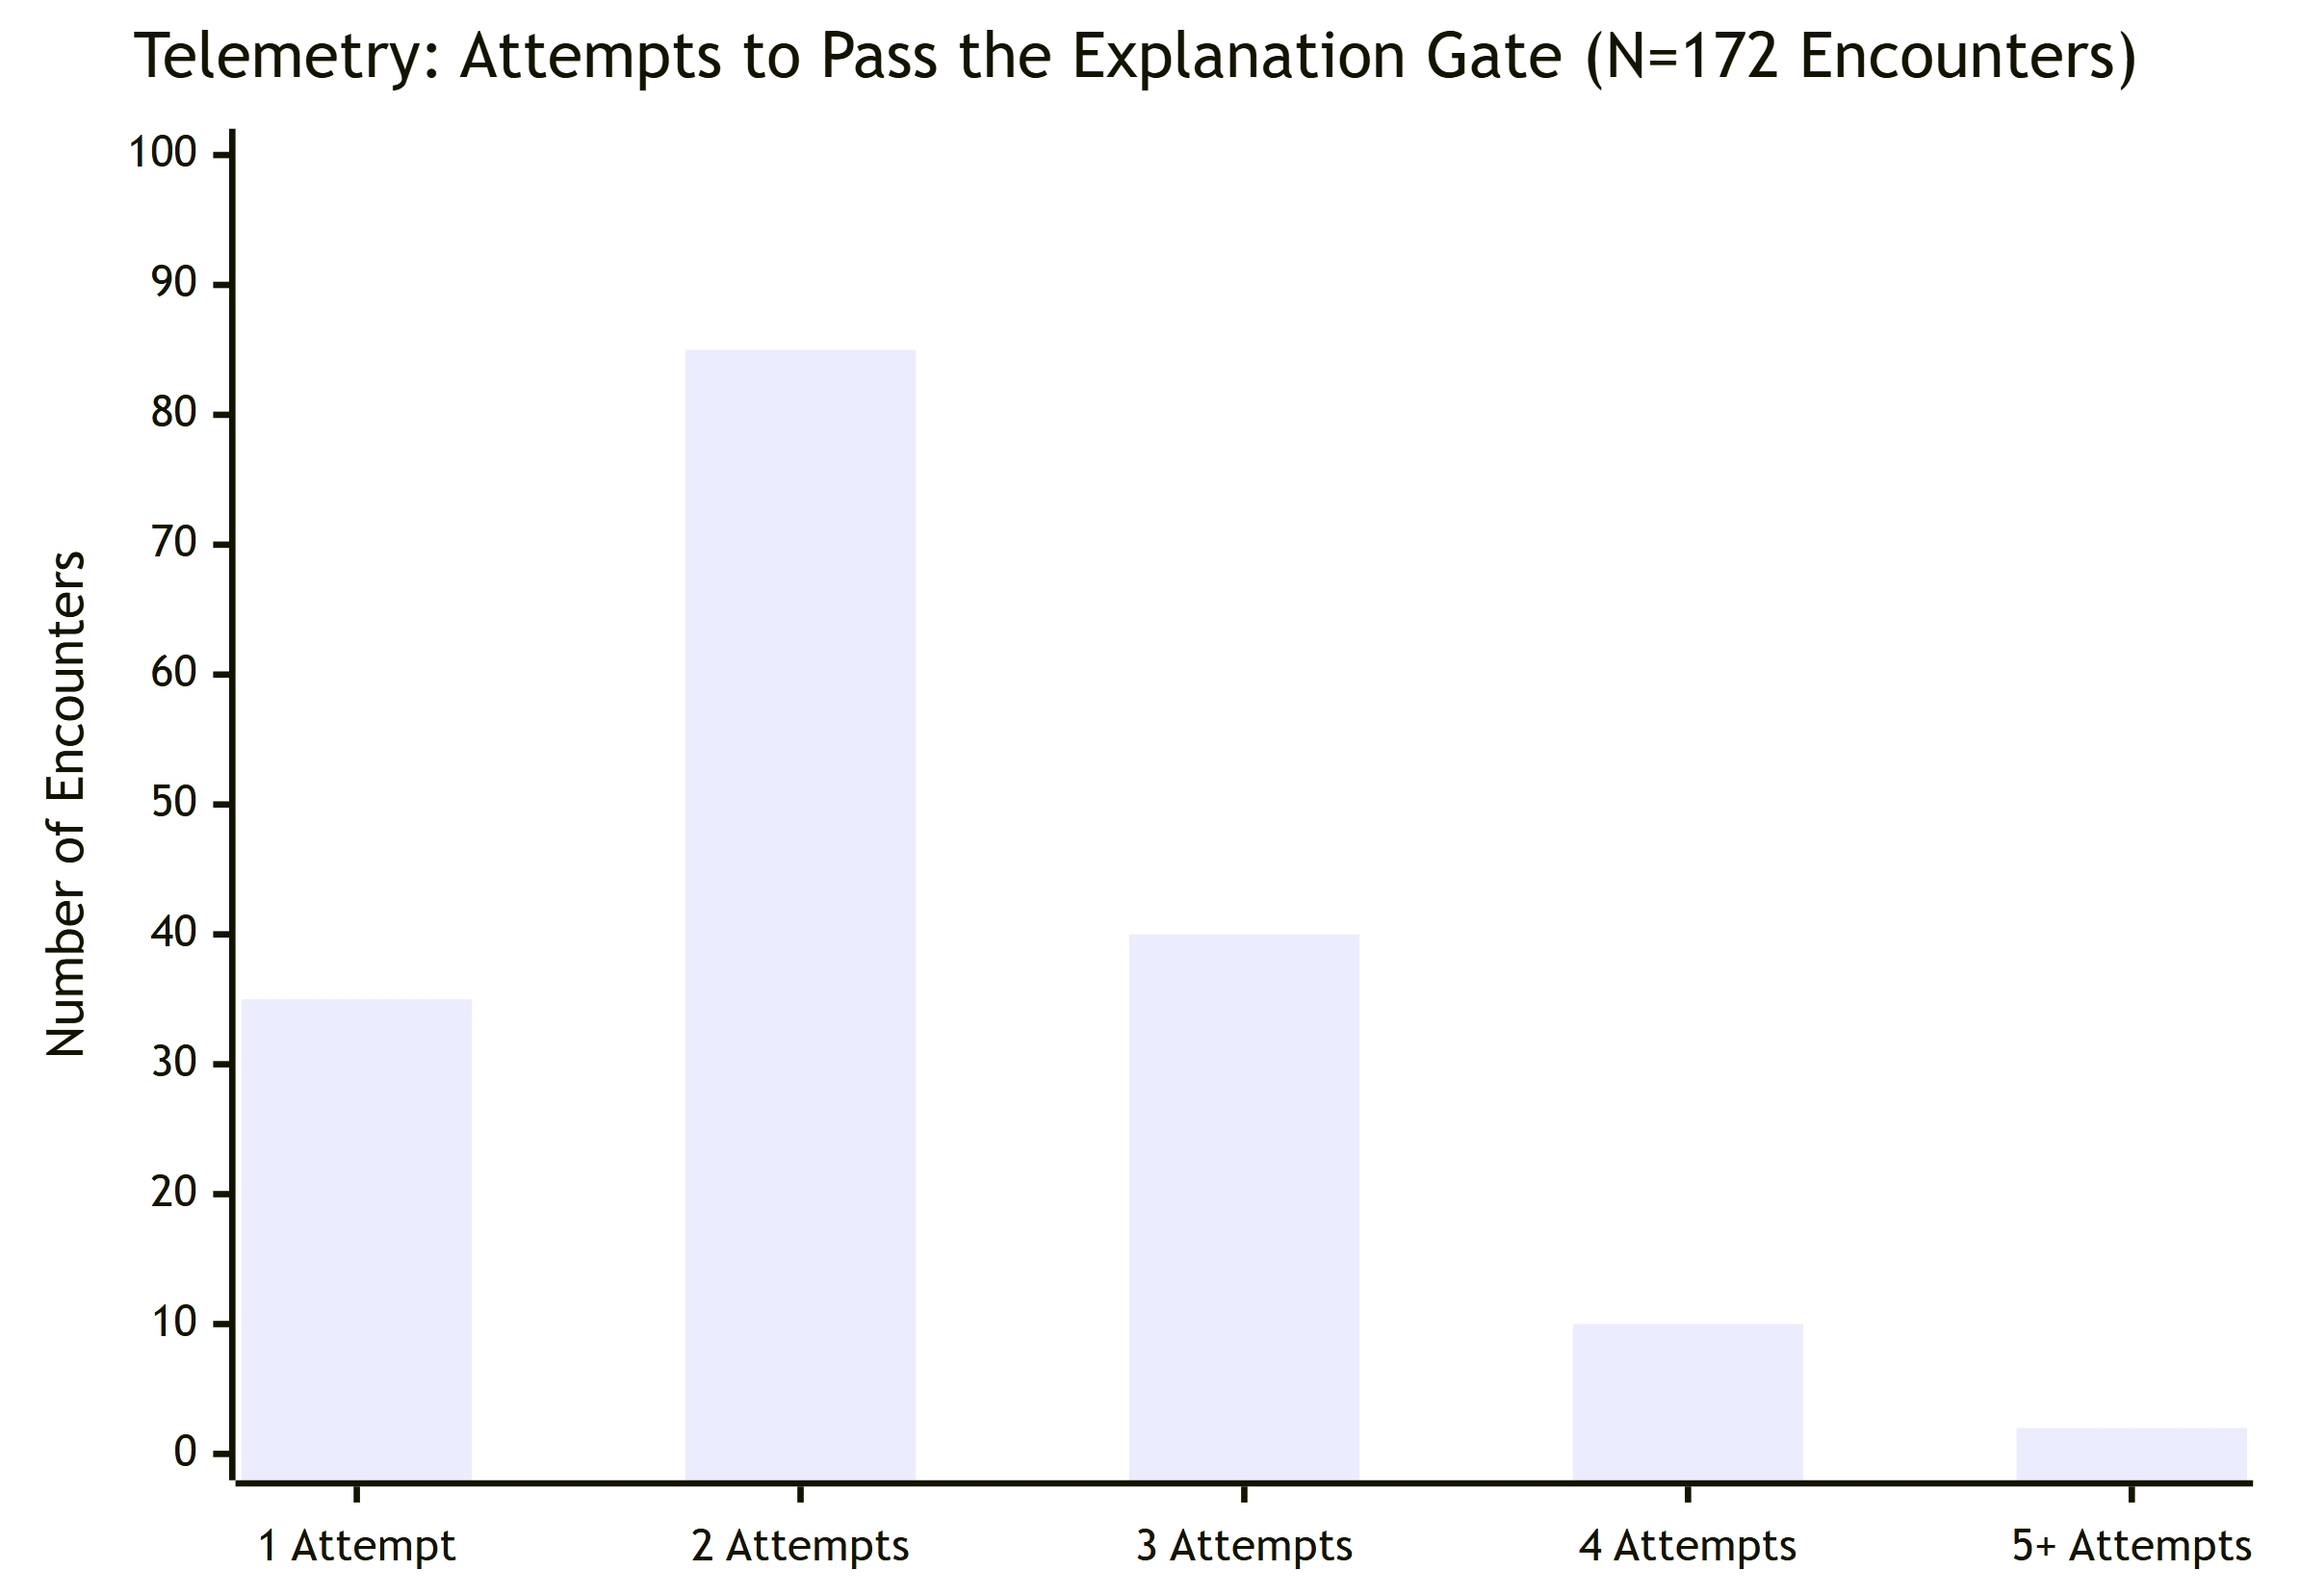
\includegraphics[width=\linewidth]{hist.jpeg}
  \caption{A histogram showing the number of attempts per Explanation Gate encounter, with a clear peak at 2 attempts}
  \label{fig:attempts_hist}
\end{figure}

\section{Discussion}

Our findings provide empirical evidence for the existence of ``Epistemic Debt'' in AI-augmented novice programming. By comparing immediate functional utility with subsequent corrective competence, we demonstrate that the efficiency gains of Generative AI can mask a significant collapse in learner comprehension if pedagogical guardrails are not enforced.

\subsection{Mapping the Cognitive Collapse: A CLT Perspective}
To understand the mechanisms behind the observed competence collapse, we mapped our Phase 1 telemetry data to the three components of Cognitive Load Theory \cite{sweller1988}.

\subsubsection{Extraneous Load}
In the Unrestricted group (B), extraneous load, i.e., the mental effort of managing syntax and IDE state, was effectively reduced to zero. While the Explanation Gate was designed to manage Germane load, our qualitative data suggests that the Scaffolded group (C) participants initially perceived it as extraneous friction. This indicates that for AI-native learners, pedagogical interventions may be misclassified as system friction, potentially leading to the ``gaming the system'' behaviors observed in specific outliers (e.g., P-55).

\subsubsection{Germane Load}
We posit that the 38.4\% success rate gap between Groups B and C is the direct result of the Explanation Gate forcing Germane Load, i.e., the effort required to build a mental schema. By requiring a ``Teach-Back'' response passing a SOLO level 3 threshold, we ensured that the learner could not integrate code without first converting the AI's outsourced logic into an offloaded mental representation. This confirms that metacognitive friction is a necessary catalyst for germane processing in generative environments.

\subsection{The False Floor of Competence and the Complexity Ceiling}
The results from Phase 1 suggest that for novice programmers, unrestricted GenAI access creates a False Floor of Competence. Group B achieved a functional utility score significantly higher than the Manual group, despite possessing arguably less cognitive ownership of the resulting codebase. These participants effectively reduced the LLM to an ``Answer Machine'' \cite{humanitarians2024answermachine}, prioritizing the retrieval of terminal outputs over the underlying procedural logic. By vibe coding their way into a degree of complexity they could not sustain, they effectively traded long-term agency for immediate velocity.

In Phase 2, this floor collapsed. The low repair success rate of the Unrestricted group suggests that when a developer treats the system as an answer machine rather than a collaborative partner, they hit a hard Complexity Ceiling. Scaling and debugging require an understanding of structural decomposition. Because Group B participants never internalized these schemas, they treated their own code as an opaque, foreign library.

\subsection{Structural Ownership of Code Artifacts}
The specific nature of the regression injected in Phase 2 (see Table \ref{tab:logic_bomb}) highlights the disconnect between \textit{visual success} and \textit{structural ownership}. By removing the \texttt{await} keyword and the rollback logic, we created a state where the application still appeared to function under ideal conditions but lacked the defensive programming required for robustness.

Participants in the Unrestricted AI group (B) were notably susceptible to this ``Visual Trap.'' Because the AI-generated code worked immediately in Phase 1, they never engaged with the underlying asynchronous architecture. When the logic bomb was injected, their troubleshooting logs showed a preoccupation with UI components rather than the data-fetching logic. They possessed what we define as ``Surface-Level Utility''; they could confirm the button existed, but they had no mental schema for the promise-based lifecycle of the enrollment event. 

In contrast, the Scaffolded group (C) was forced to explain this exact lifecycle to the Judge API during construction. By articulating the relationship between the \texttt{fetch} request and the state update, they performed the necessary germane processing to ``buy back'' their epistemic debt. When the bug was injected, these participants did not simply debug; they recognized a structural regression in a system they now cognitively owned. This suggests that metacognitive friction acts as an architectural audit, forcing the developer to move beyond the ``vibe'' of a working UI to the reality of the underlying implementation.

\subsection{Industry Implications: Realization of Epistemic Debt}
The risks identified in our laboratory setting find a direct parallel in recent industry events, validating the Epistemic Debt hypothesis at scale. The \textbf{Clawdbot/Moltbot incident} of early 2026 \cite{reuters2026moltbot} serves as a primary case study of the dangers of high utility coupled with low corrective competence. In that event, thousands of developers deployed personal AI agents using generated configurations they did not fully understand. 

While the users successfully orchestrated the functional intent, they outsourced the implementation details, specifically the binding of insecure WebSocket ports. When these systems were scanned by malicious actors, the vibe coders were helpless to intervene. Much like the participants in our Unrestricted group, these developers were effectively Senior Architects in capability but Junior Interns in comprehension. Without the foundational mental models required for security and architectural oversight, the functional utility they achieved was fundamentally fragile.

\subsection{Fragile Velocity vs. Sustainable Velocity}
A common critique of metacognitive interventions is that they impede development speed. However, our data suggests this is a false dichotomy. While the Explanation Gate introduced a time penalty of approximately 14 minutes in Group C, this cost was largely subsidized by the generation speed of the LLM. 

We frame this trade-off as a shift from \textbf{Fragile Velocity} to \textbf{Sustainable Velocity}. The \textit{VibeCheck} intervention ensures that the velocity gained through AI is maintainable by the human developer. By enforcing the ``Teach-Back'' protocol, the tool ensures that the intrinsic load of the task is offloaded rather than outsourced.

\subsection{Self-Scaffolding and Interactional Stances}
The outlier analysis in RQ3 provides a final, critical insight: accumulation of Epistemic Debt is not solely a function of the tool, but of the user's \textit{interactional stance}. Successful participants in the Unrestricted group naturally adopted a ``Consultant Stance.'' This suggests that while advanced learners may possess the metacognitive discipline to treat AI as a peer, novices require structural friction to prevent them from falling into the ``Contractor Stance.'' 

Future learning systems must, therefore, move beyond passive code generation toward active metacognitive mediation. By automating the verification of student explanations through an LLM-as-a-Judge framework \cite{choma2025}, we can scale such interventions to meet the demands of learners in the current GenAI era.

\section{Threats to Validity}

\subsection{Internal Validity}
A primary threat is the \textbf{Hawthorne Effect}; participants knew they were in a monitored study, which may have artificially increased their persistence in the Scaffolded group. To mitigate this, we anonymized the Judge's feedback to appear as standard IDE warnings rather than ``test" feedback. Furthermore, the 90-minute limit for Phase 1 was chosen to simulate the time pressure of a standard technical screen, grounding the velocity results in professional reality. Nevertheless, the limitation remains, despite our mitigation strategies.

\subsection{External Validity}
Our study focused exclusively on \textbf{novice programmers} (students and bootcampers). It is possible that for expert developers, who already possess robust internal mental models, the Explanation Gate would represent purely extraneous load with no germane benefit. The ``Epistemic Debt" we observed is likely a function of the \textit{novice-AI dyad}, and results may not generalize to experienced programmers who utilize AI for boilerplate tasks rather than core logic. In either case, approaching the problem from first principles, i.e., defining germane, intrinsic and extrinsic loads will allow for the delineation of offloading and outsourcing for the respective populations, and designing appropriate scaffolds, as a result. We posit that our study, grounded in cognitive load theory, while not externally face valid nevertheless provides directional support for the design of scaffolds for experienced programmers as well.

\subsection{Construct Validity}
We used ``Repair Success" as a proxy for \textbf{Corrective Competence}. Critics might argue that this measures debugging skill rather than understanding. However, as noted in Section 3.4.2, because the bug was a regression of the user’s \textit{own} code integrated moments prior, we believe it remains a valid measure of cognitive ownership.

\section{Conclusion}
This study has demonstrated that the democratization of software creation via GenAI carries the latent risk of an industry-wide collapse of competence. However, this breakdown is not inevitable. By deliberately introducing \textbf{Metacognitive Friction} into the development loop, we can leverage the immense productivity gains of LLMs while ensuring that the humans at the helm remain capable of maintaining the complex systems they build. To prevent the mass production of unmaintainable software, we must ensure that the price of velocity is not the loss of comprehension.

\section{Future Work}

The findings of this study open several avenues for investigating the long-term sustainability of AI-assisted learning environments. We identify four primary areas for future research:

\subsection{Adaptive Scaffolding and Instructional Fading}
The current implementation of the \textit{VibeCheck} Explanation Gate utilizes a static threshold (SOLO Level 3). Future work should explore \textit{adaptive friction}, where the complexity of the required explanation ``fades" as the system detects increasing learner competence. Drawing on the Expertise Reversal Effect \cite{kalyuga2009expertise}, a system that transitionally moves from high-friction scaffolds to frictionless utility could prevent the ``Fragile Expert" syndrome while eventually granting the developer the high-velocity benefits of an unrestricted environment.

\subsection{Longitudinal Learning and Mental Model Decay}
Our experiment measured corrective competence immediately following a construction task. However, the long-term persistence of schemas formed under metacognitive friction remains unknown. Future longitudinal studies should investigate whether ``buying back" epistemic debt through teach-back protocols leads to higher retention of architectural principles over months of professional practice, or if the ``Consultant Stance" naturally erodes as users face the time-pressures of industrial production.

\subsection{Collaborative Human-AI-Human Systems}
While this study focused on the programmer-AI dyad, modern software engineering is a social activity. Research is needed to determine how epistemic debt impacts code reviews and collaborative debugging. If a senior developer reviews code authored by a novice ``Vibe Coder," does the lack of cognitive ownership in the junior dev create a bottleneck in the team's collective corrective competence? Extending the Explanation Gate to include collaborative ``Teach-Forward" protocols between humans could mitigate these social bottlenecks.

\subsection{Equity, Diversity, and the AI Experience Gap}
A critical area for future inquiry is the impact of Generative AI on underrepresented groups in Computer Science. Currently, Black and Hispanic students earn close to 20\% of CS degrees in the United States, combined, \cite{siek2025taulbee,nces2023digest} yet they often report higher rates of ``imposter syndrome" and lower access to early-career mentorship. Generative AI has the potential to act as a ``leveling agent"; however, if unrestricted AI usage leads to a disproportionate accumulation of epistemic debt among learners with less existing social capital, it may inadvertently widen the ``competence gap" during technical interviews. Future research must quantify whether scaffolded AI tools like \textit{VibeCheck} provide a more equitable pathway to senior-level architectural understanding for students from diverse socio-economic and racial backgrounds.

\section*{Artifact Availability}
  The \textit{VibeCheck} VS Code/Cursor extension, the Course Scheduler experimental task suite (starter scaffold, reference implementation, 12-assertion Puppeteer grading harness, and logic bomb version), and the complete three-condition study replication protocol are openly available at
  \begin{sloppypar}
  \url{https://github.com/sreecharansankaranarayanan/vibecheck}
  \end{sloppypar}

\bibliographystyle{ACM-Reference-Format}
\bibliography{references}

\end{document}